\chapter{Die Problemstellung}
\label{sec:prob}
	
	Dieses Kapitel soll eine grobe Einführung in die Thematiken Bildverarbeitung und \gls{ocr} bieten und ferner die Motivation für diese Arbeit im Zusammenhang mit der Segmentierung von Bildern aufzeigen. Bei alledem werden auch mögliche Schwierigkeiten bei diesem Vorgang mit in den Blick genommen.
	
	\section{Grundlegendes über Bildverarbeitung}
	\label{sec:bild-basics}
	
		Was ist Bildverarbeitung? - Um diese Frage zu beantworten, wird das Buch \textit{Digital Image Processing} von Rafael C. Gonzalez und Richard E. Woods \cite[S. 1--3]{gonzalez-woods} herangezogen. Die Autoren konstatieren, dass die Meinungen hierzu unter den Fachleuten auseinandergehen. Präzise ausgedrückt, liegt die Meinungsverschiedenheit in der Frage nach der Grenze zwischen der Bildverarbeitung und damit verwandten Bereichen, z.B. dem maschinellen Sehen. Gonzalez und Woods versuchen deshalb, ihre eigene Definition aufzustellen, die hier zum Zwecke der Veranschaulichung ausreichen soll. So beginnen sie damit, eine Unterscheidung von rechnergestützten Prozessen wie folgt vorzunehmen: 
		\begin{description}
			\item[Low-Level] Darunter fallen einfache Operationen direkt am Bild, wie zum Beispiel Rauschreduktion oder die Erhöhung des Kontrastes, oder aber auch simple arithmetische Operationen. Input sowie Output sind jeweils durch ein Bild gegeben.
			\item[Mid-Level] Diese Kategorie von Prozessen zeichnet sich dadurch aus, dass aus einem Bild bestimmte Eigenschaften/Bereiche extrahiert werden, um daraus eine Information zu gewinnen. Während die Eingabe aus einem ganzen Bild besteht, beläuft sich die Ausgabe lediglich auf einen Teil davon bzw. ein bestimmtes Attribut des Bildes. Exemplarisch hierfür kann die Segmentierung angeführt werden, die in dieser Arbeit mit Hilfe der in Abschnitt \ref{sec:de} vorgestellten Methode realisiert werden soll. Bei der Segmentierung wird das Bild in Sub-Bilder eingeteilt, bis die für die jeweilige Anwendung interessante Region klar abgegrenzt im Bild erscheint.
			\item[High-Level] Hier werden die aus den Mid-Level Prozessen erhaltenen Informationen verwendet, um bestimmte Aktionen auszulösen (z.B. im Bezug auf maschinelles Sehen).
		\end{description}
	
		Auf dieser Grundlage fassen Gonzalez und Woods alle Low- und Mid-Level Prozesse zusammen und deckeln dies unter dem Begriff Bildverarbeitung. \\
		
		Ein Bild in diesem Kontext kann aus mathematischer Sicht als eine Funktion $f(x, y)$ von zwei Variablen begriffen werden, die an der Stelle $(x, y)$ etwas zurückliefert, der als \textit{Intensität} interpretiert wird. Diese kann, je nach Farbsystem, entweder ein Skalar (schwarz-weiß) oder ein Tupel von Werten (\textbf{R}ed-\textbf{G}reen-\textbf{B}lue: 3-Tupel, nachzulesen bei \cite{rgb-info}) sein. 
	
		\glsreset{ocr}
	
	\section{\gls{ocr} und Segmentierung}
	\color{red} [Bild beschreiben] \color{black}
	
		\begin{figure}[H]
			\centering
			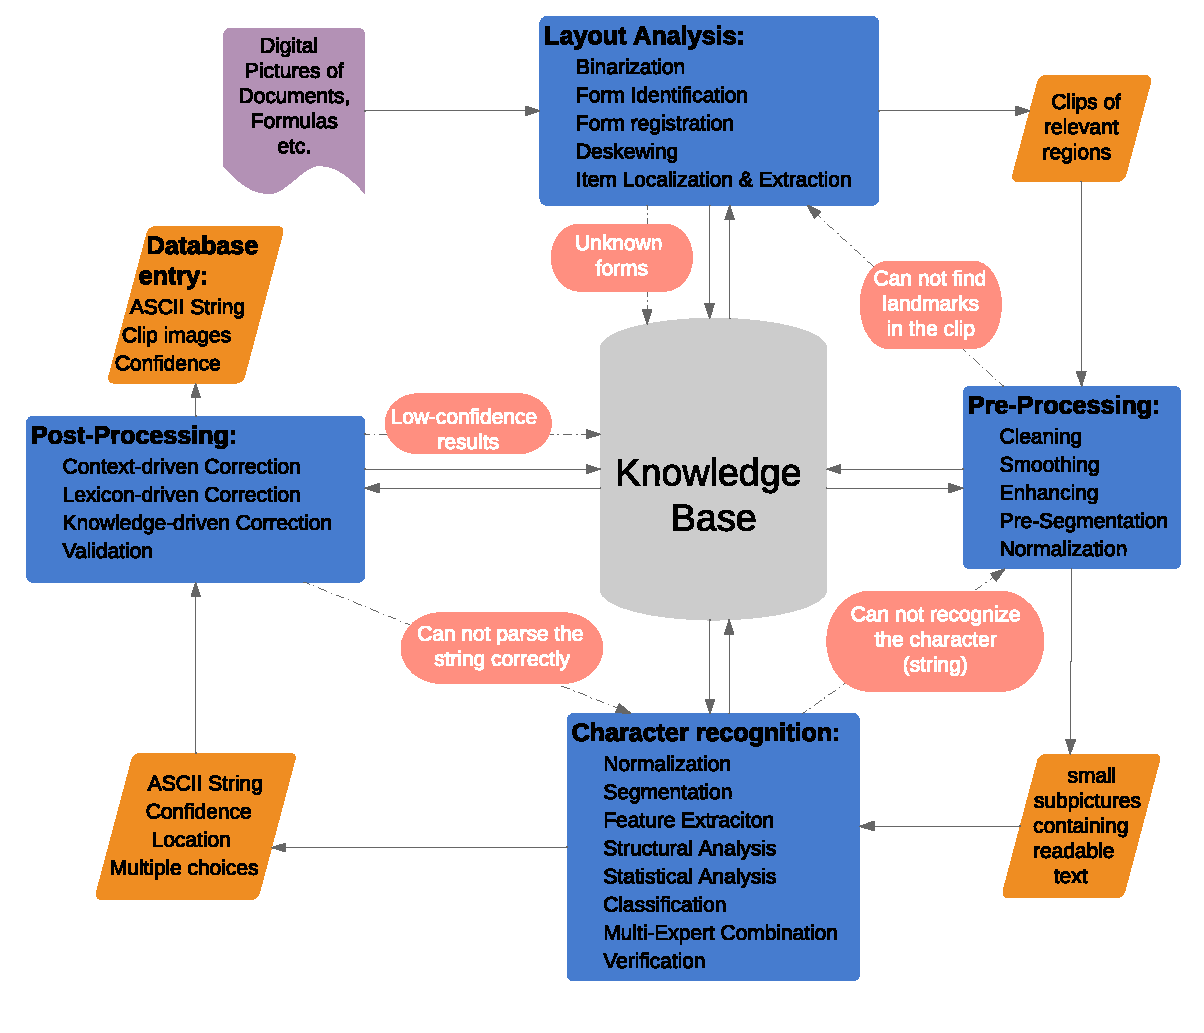
\includegraphics[width=\linewidth]{Ablauf-OCR_Cheriet-et-al.pdf}
			\caption[typisches \gls{ocr}-Ablaufschema]{Schematische Darstellung des 
				Ablaufs in einem intelligenten \gls{ocr}-System (Nachbildung aus 
				\cite[Seite 7]{cher-et-al-ocr})}
			\label{fig:ocr-system}
		\end{figure}
	
		Einen in der heutigen Zeit zentralen Anwendungsfall für die Bildverarbeitung stellt \gls{ocr} dar. Wie der Name bereits vermuten lässt, ist das Ziel der \gls{ocr}, Zeichen oder Formen aus digitalen Bildern zu extrahieren und weiterzuverarbeiten. Schon in den frühen 1950ern - so bei \cite{cher-et-al-ocr} - haben Forscher nach Möglichkeiten gesucht, auf Papier befindlichen Text mit Hilfe von Rechnerkapazitäten einzulesen, um dem Menschen die mühselige Arbeit des manuellen Abtippens von Dokumenten abzunehmen.

		Damit ein System, wie es auf Abbildung \ref{fig:ocr-system} zu 
		erkennen ist, zuverlässig Zeichen erkennen kann, muss es unter 
		anderem auf die Formen der Zeichen trainiert werden und als Input ein für 
		die Anwendung angemessen segmentiertes Bild erhalten. In Abbildung \ref{fig:seg-example-good} lässt sich an einem Beispiel betrachten, was die Segmentierung eines Bildes bewirkt, wobei dies ein Beispiel für eine gute Segmentierung ist - also eine Segmentierung, nach der der Text im Bild korrekt und vollständig gelesen werden konnte:
		\begin{figure}[H]
			\centering
			\subfloat[][unsegmentiertes OriginalBild]{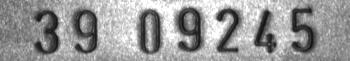
\includegraphics[width=0.48\linewidth]{IMG_3909245}}
			\qquad
			\subfloat[][segmentiertes Bild]{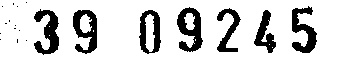
\includegraphics[width=0.48\linewidth]{IMG_3909245-seg-good}}
			\caption{Segmentierung an einem Beispiel (Einteilung in zwei Klassen) - gutes Beispiel}
			\label{fig:seg-example-good}
		\end{figure}
		Dem gegenübergestellt wird ein Exempel einer schlechten Segmentierung in Abbildung \ref{fig:seg-example-bad}:
		\begin{figure}[H]
			\centering
			\subfloat[][unsegmentiertes OriginalBild]{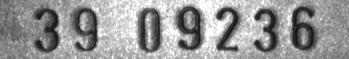
\includegraphics[width=0.48\linewidth]{IMG_3909236}}
			\qquad
			\subfloat[][segmentiertes Bild]{
\includegraphics[width=0.48\linewidth]{IMG_3909236-seg-bad}}
			\caption{Segmentierung an einem Beispiel (Einteilung in zwei Klassen) - schlechtes Beispiel}
			\label{fig:seg-example-bad}
		\end{figure}
		Wie auf Abbildung \ref{fig:seg-example-bad}b unschwer zu erkennen ist, werden zu viele Pixel in der Umgebung des ersten und letzten Zeichens schwarz gefärbt, was die Konturen dieser beinahe verschwinden lässt und so dafür sorgt, dass der auf Abbildung \ref{fig:seg-example-bad}a dargestellte Text nicht korrekt erkannt werden kann.\\
		Wie im Buch \cite[Kapitel 10]{gonzalez-woods} von Gonzalez und Woods nachgelesen werden kann, gibt es mehrere Arten, um eine Segmentierung zu realisieren: \textit{Thresholding}, \textit{Edge-Based-Segmentation} und \textit{Region-Based-Segmentation}. Sowohl aus erstgenannter als auch aus letztgenannter Gruppe von Segmentierungsmethoden wird jeweils ein möglicher Ansatz in den Paragraphen \ref{sec:meth1} und \ref{sec:meth2} eingehend vorgestellt sowie im weiteren Verlauf dieser Arbeit zur Generierung der Ergebnisse in Kapitel \ref{sec:results} herangezogen. \\
		%Allen Methoden ist gemein, dass im Vorfeld festgelegt werden muss, in wie viele Klassen $K$ das Bild eingeteilt werden soll. 
		
	\subsection{Modell 1: Gaußsche Annäherung an das Histogramm}
	\label{sec:meth1}
		
		Dieses Vorgehen aus der Gruppe der \textit{Thresholding}-Methoden basiert auf der Arbeit von Erik Cuevas und seinen Kollegen \cite{cuevas-meth1} und zielt darauf ab, das Histogramm eines Bildes mittels einer Summe von Gaußschen Wahrscheinlichkeitsfunktionen zu approximieren und den Fehler zwischen diesen beiden Funktionen zu minimieren.
		
		Unter der Annahme, dass ein Graustufenbild vorliegt - also die in Abschnitt \ref{sec:bild-basics} erwähnte Bildfunktion $f(x,y)$ einen Wert im Intervall $[0, ..., L-1]$ zurückliefert, mit $L = $ Anzahl der Graustufen - ergibt sich das Histogramm eines Bildes nach Gleichung \ref{eq:histogram} zu
		\begin{flalign}
			\centering
			h(g) &= \frac{n_{g}}{N} \label{eq:histogram}
		\end{flalign}
		dabei steht $n_{g}$ für die Anzahl an Pixel mit der Graustufe $g$, während $N$ die Gesamtzahl aller Pixel im Bild repräsentiert.\\
		Dieses Histogramm kann dann näherungsweise über die Summe von Gaußschen Wahrscheinlichkeitsdichtefunktionen, wie in Gleichung \ref{eq:gauss-sum} dargestellt, angegeben werden:
		\begin{flalign}
			\centering
			p(x) = \sum_{i=1}^{K} P_{i} \cdot p_{i}(x) \quad \textrm{mit} \quad p_{i}(x) = \frac{1}{\sigma_{i}\sqrt{2\pi}} \exp\left(-\frac{1}{2} \cdot \left(\frac{x - \mu_{i}}{\sigma_{i}}\right)^{2}\right), \label{eq:gauss-sum}
		\end{flalign}
		unter der Voraussetzung, dass $K$ die Anzahl der Klassen, in die das Bild aufgeteilt werden soll, und $P_{i}$ die Wahrscheinlichkeit dafür darstellt, dass ein zufällig gewählter Grauwert $x$ innerhalb der Klasse $i$ liegt. Weiterhin ist $p_{i}(x)$ die der Klasse $i$ zugehörige Komponente der Approximation $p(x)$ in Form einer Gaußschen Dichtefunktion, jedoch wurde die Formel aus \cite{papula-gauss} entnommen, da die Darstellung in \cite{cuevas-meth1} fehlerhaft ist (das $\sigma_{i}$ im ersten Bruch befindet sich innerhalb der Quadratwurzel). Zusätzlich ist $\sigma_{i}$ als Standardabweichung und $\mu_{i}$ als Mittelwert angegeben.\\
		Nun sind die Parameter $\sigma_{i}$, $\mu_{i}$ und $P_{i}$ mit $i = 1, ..., K$ so zu bestimmen, dass nachstehendes Problem
		\begin{flalign}
			\centering
			\underset{P_{i}, \mu_{i}, \sigma_{i}}{arg \ min} \ E \quad \textrm{mit } E = \frac{1}{n} \sum_{j=1}^{n}[p(x_{j}) - h(x_{j})]^{2} + \omega \cdot \left| \left( \sum_{i=1}^{K} P_{i} \right) - 1 \right| \label{eq:mean-square-error}
		\end{flalign}
		gelöst wird - ausgehend von der Graustufenanzahl $n$ und dem Penalty-Faktor $\omega$, der sich genau dann auswirkt, wenn die Bedingung $\sum_{i=1}^{K} P_{i} = 1$ nicht erfüllt ist.\\
		Die Minimierung einer solchen Funktion erweist sich laut \cite{cuevas-meth1} als ein komplexes Problem. Eine analytische Lösung erfordert, wie in \cite[S. 248-250]{papula-optimization} anschaulich dargelegt, die jeweiligen partiellen Differentiationen der Funktion in Gleichung \ref{eq:mean-square-error} nach den Parametern $\sigma_{i}$, $\mu_{i}$ und $P_{i}$ zu bestimmen und gleich Null zu setzen. Dies führt auf ein Gleichungssystem mit $3K$ Unbekannten und $3K$ Gleichungen der Form
		\begin{flalign*}
			\textrm{\color{red} Formeln für partielle Ableitungen hier einfügen}
		\end{flalign*}
		Nach den in \cite[S. 26]{papula-alg-eq} aufgestellten Kriterien für die Linearität eines Gleichungssystems ist obiges ein \textit{nichtlineares} Gleichungssystem und somit analytisch bestenfalls mit erheblichem Aufwand lösbar \color{red}[muss noch belegt werden]\color{black}. In solchen Fällen wird dann ein numerisches Verfahren zur Approximation einer Lösung in annehmbarer Zeit herangezogen, beispielsweise jenes, das in Abschnitt \ref{sec:de} behandelt wird. 
		
		Im Folgenden soll zur weiteren Erläuterung des Modells davon ausgegangen werden, dass die Kenngrößen $\sigma_{i}$, $\mu_{i}$ und $P_{i}$ im Sinne von Gleichung \ref{eq:mean-square-error} bereits ermittelt wurden. \\
		Der letzte Schritt, um hieraus schließlich die Threshold-Werte $T_{1}, ... , T_{K-1}$ zu erhalten, führt über die Lösung der folgenden quadratischen Gleichung:
		\begin{flalign}
			AT_{i^{2}} + BT_{i} + C &= 0 \label{eq:quad-eq-thresh}
		\end{flalign}
		mit den Koeffizienten
		\begin{flalign}
			A &= \sigma_{i}^{2} - \sigma_{i+1}^{2}, \notag \\
			B &= 2 \cdot (\mu_{i}\sigma_{i+1}^{2} - \mu_{i+1}\sigma_{i}^{2}), \notag \\
			C &= (\sigma_{i}\mu_{i+1})^{2} - (\sigma_{i+1}\mu_{i})^{2} + 2 \cdot (\sigma_{i}\sigma_{i+1})^{2} \cdot \ln \left(\frac{\sigma_{i+1}P_{i}}{\sigma_{i}P_{i+1}}\right) \notag
		\end{flalign}
		Wie sich diese im Einzelnen zusammensetzen, soll an dieser Stelle nicht erläutert werden, lässt sich jedoch bei \cite[S. 13+14]{cuevas-meth1} nachlesen.
		
		Anhand der so ermittelten Threshold-Werte werden nun alle Pixel des Bildes mittels untenstehender Gleichung aus \cite[S. 739]{gonzalez-woods} zugeordnet:
		\begin{flalign}
			\centering
			g(x, y) = 
			\begin{cases}
				a_{1} & \textrm{if } f(x, y) > T_{K-1}\\
				a_{2} & \textrm{if } T_{K-2} < f(x, y) \leq T_{K-1}\\
				... \\
				a_{K} & \textrm{if } f(x, y) \leq T_{1}
			\end{cases}
			\label{eq:threshold}
		\end{flalign}
		Dabei sind $a_{1}, ..., a_{K}$ voneinander unterschiedliche Graustufenwerte.
	
	\subsection{Modell 2: K-Means}
	\label{sec:meth2}
	
		Der K-Means-Algorithmus wurde 1967 von James B. MacQueen \cite{macqueen-kmeans} vorgestellt und wird heute noch häufig zur Gruppierung großer Datenmengen eingesetzt - so in \cite{kmeans-info} zu lesen.\\
		Die grundlegende Idee hinter K-Means besteht in der Generierung von Mittelpunkten als Repräsentanten für verschiedene Bereiche in einem Datensatz. 
		\begin{definition}
			\label{def:kmeans1}
			Gegeben sei eine Folge von Messpunkten $x_{j} \in \mathbb{R}^{d},$ $j \in [1,n]$, wobei $n$ gleich der Anzahl der Messpunkte ist und $d$ für die Dimension dieser steht. Dann existiert eine Segmentierung $S = \{S_{1}, ..., S_{K}\}$
		\end{definition}